\documentclass[12pt]{article}
\usepackage[utf8]{inputenc}
\usepackage[spanish]{babel}
\usepackage{graphicx}
\usepackage{float}
\title{Práctica 3\\Programación Evolutiva}
\author{Grupo 01\\Rafael Fernández López\\Ángel Valero Picazo}
\date{}

\pdfinfo
{
  /Title       (PRACTICA3-PE)
  /Author      (RAFAEL FERNANDEZ LOPEZ, ANGEL VALERO PICAZO)
}

\begin{document}

\maketitle
\newpage
\newpage
\tableofcontents
\newpage

\section{Introducción}

	En esta memoria se van a estudiar los diferentes métodos de selección para poder
    evaluar cuáles se comportan mejor y cuáles son menos precisos a la hora de tratar el problema del
    multiplexor implementado en esta práctica.


\section{Cruce}

	El algoritmo de cruce varia respecto al de otras practicas, ya que aquí se trabaja con arboles. Esta estructura arbórea conlleva el problema de poder cruzar tanto en funciones(nodos) como en términos(hojas), para poder realizar cruces relevantes y conlleven a una buena solución se le da mas probabilidad de cruce a las funciones que a los términos, en nuestro caso un 90\% para funciones y un 10\% para términos. 

\section{Mutación}

	El algoritmo de mutación también se ve afectado por la nueva representación arbórea de la práctica. En la mutación sucede algo parecido al cruce ya que al tener funciones y términos pueden mutar indistintamente unos u otros. En nuestra implementación se mira cada uno y dependiendo si es función o termino se muta de distinta manera, para las funciones se comprueba que tipo de operador contiene: si es NOT lo eliminamos, si es AND se cambia por una OR y viceversa y si es IF se niega el termino de control de dicho IF. En el caso de los términos se cambia el 0 por 1 y viceversa.

\section{Estudio de los diferentes parámetros del Algoritmo Genético con selección por Torneo}

	Estudio realizado con selección por torneo. Se han ido variando los diferentes parámetros, por defecto hemos tomados los siguientes valores:(suponemos que se permite la utilización de IF)

%tabla
\begin{table}[H]
\begin{center}
\begin{tabular}{|cc|} \hline
Tamaño de la Población   & 150  \\  
Número Máximo de Generaciones  &  150 \\
Probabilidad de Cruce & 0.6 \\
Probabilidad de Mutación & 0.1 \\
Porcentaje de Elitismo & 0.1 \\
Profundidad & 3 \\ \hline
\end{tabular}
\end{center}
\end{table}


\subsection{Tamaño de la Población}

%tabla
\begin{table}[H]
\begin{center}
\begin{tabular}{|ccccc|} \hline
Tamaño	   & 50 & 100 & 150 & 200 \\  \hline
Resultado  & 52  & 56 &  56 &  64\\ \hline
\end{tabular}
\end{center}
\end{table}

\begin{figure}[H]
\centering
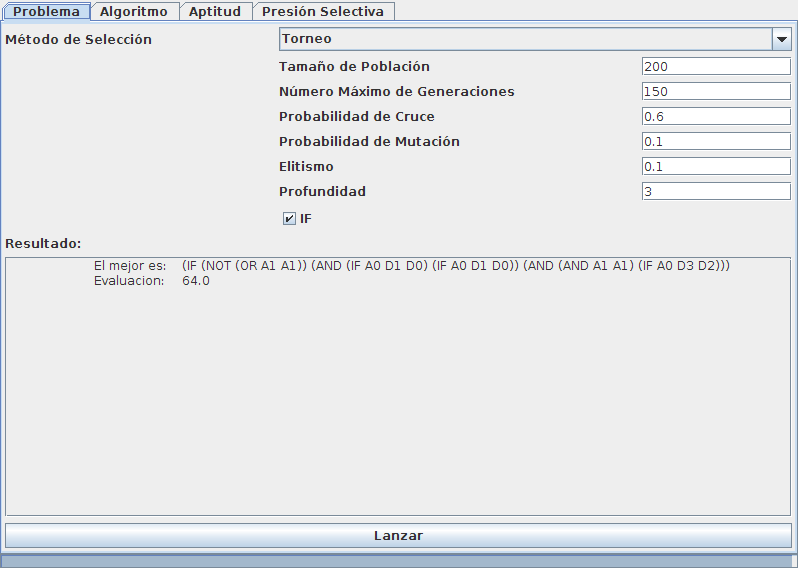
\includegraphics[scale=0.4]{graficas/tp64}
\caption{Captura mejor resultado.}
\end{figure}

\begin{figure}[H]
\centering
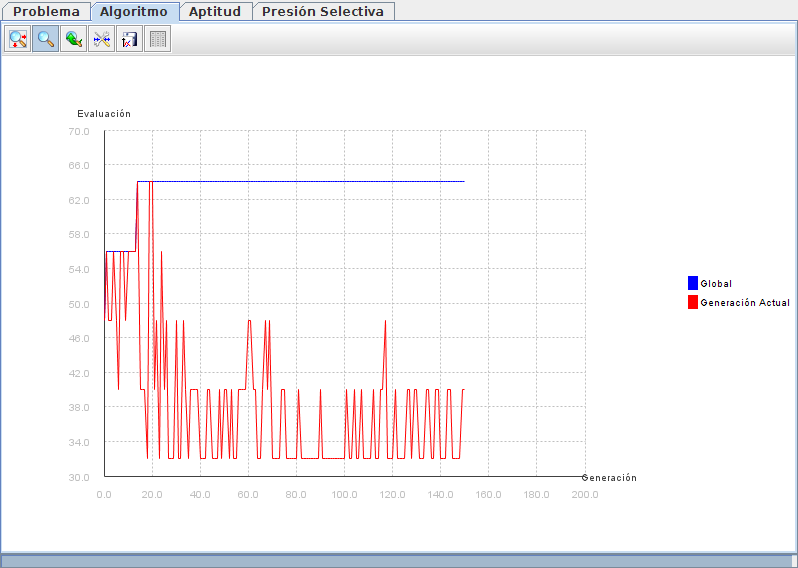
\includegraphics[scale=0.4]{graficas/tpg64}
\caption{Gráfica mejor resultado.}
\end{figure}

Podemos apreciar en la gráfica que contra mayor es el tamaño de población más se acerca al mejor resultado posible. De esta manera podemos decir que 200 de tamaño de población es una buena cifra para trabajar con el algoritmo conservando la eficiencia. 

	

\subsection{Número Máximo de Generaciones}
%tabla
\begin{table}[H]
\begin{center}
\begin{tabular}{|ccccc|} \hline
Num Generaciones  & 100 & 200 & 300 & 400 \\  \hline
Resultado  & 56  & 56 & 56 & 56 \\ \hline
\end{tabular}
\end{center}
\end{table}

\begin{figure}[H]
\centering
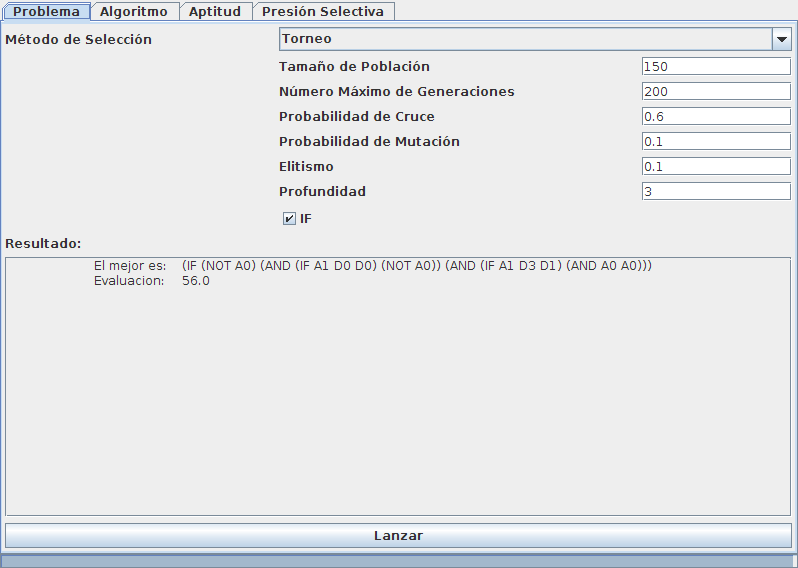
\includegraphics[scale=0.4]{graficas/nm56}
\caption{Captura mejor resultado.}
\end{figure}

\begin{figure}[H]
\centering
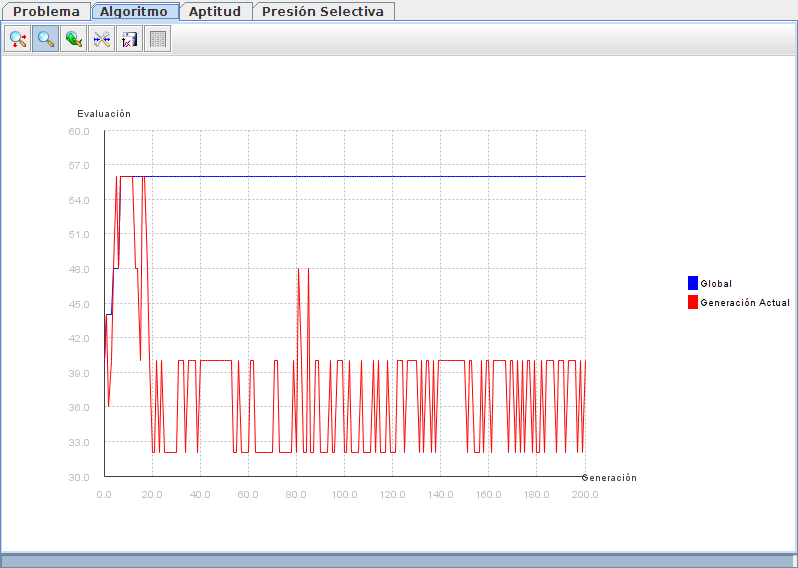
\includegraphics[scale=0.4]{graficas/nmg56}
\caption{Gráfica mejor resultado.}
\end{figure}

En este caso al variar el número máximo de generaciones el resultado no experimenta grandes cambios y se mantiene mas o menos constante, cabe destacar que para una mayor eficiencia un resultado óptimo podría ser elegir el intervalo de 100 a 200.	

	

\subsection{Probabilidad de Cruce}
%tabla
\begin{table}[H]
\begin{center}
\begin{tabular}{|ccccc|} \hline
Probabilidad   & 0.2 & 0.4 & 0.5 & 0.7 \\  \hline
Resultado  & 48  & 52 & 52 & 64 \\ \hline
\end{tabular}
\end{center}
\end{table}

\begin{figure}[H]
\centering
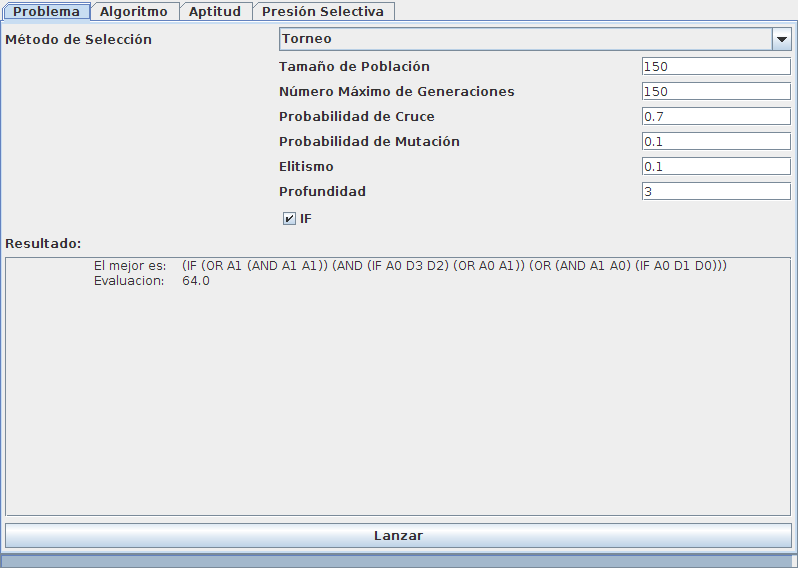
\includegraphics[scale=0.4]{graficas/pc64}
\caption{Captura mejor resultado.}
\end{figure}

\begin{figure}[H]
\centering
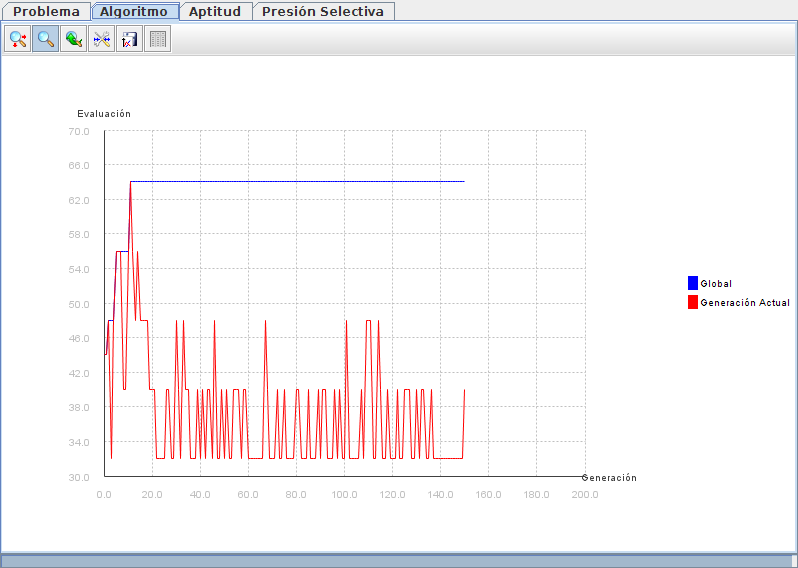
\includegraphics[scale=0.4]{graficas/pcg64}
\caption{Gráfica mejor resultado.}
\end{figure}

Relativo a la probabilidad de cruce se puede observar la mejora que sufre el resultado de nuestro algoritmo al ir aumentando poco a poco la probabilidad de cruce hasta llegar a 0.7 que es un buen valor para poder conseguir buenos resultados.	

	

\subsection{Probabilidad de Mutación}
%tabla
\begin{table}[H]
\begin{center}
\begin{tabular}{|ccccc|} \hline
Probabilidad   & 0.05 & 0.1 & 0.15 & 0.2 \\  \hline
Resultado  &  60 & 56 & 56 & 52 \\ \hline
\end{tabular}
\end{center}
\end{table}

\begin{figure}[H]
\centering
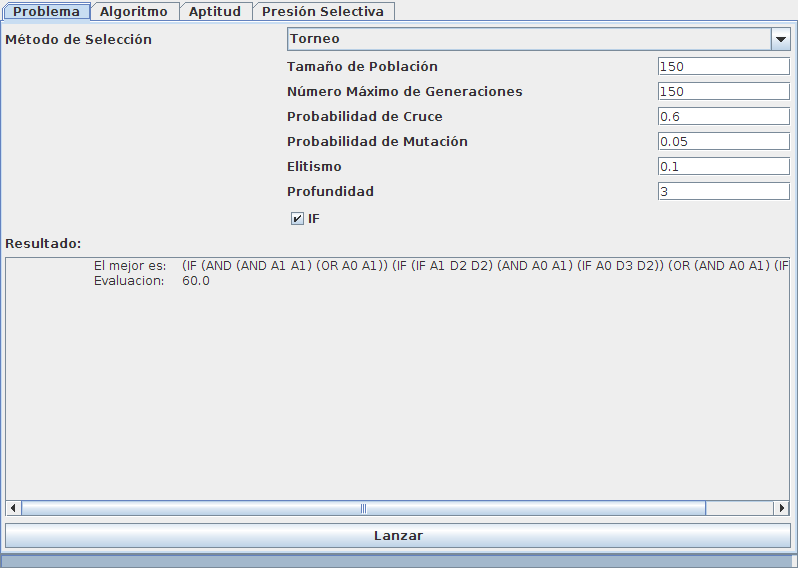
\includegraphics[scale=0.4]{graficas/pm60}
\caption{Captura mejor resultado.}
\end{figure}

\begin{figure}[H]
\centering
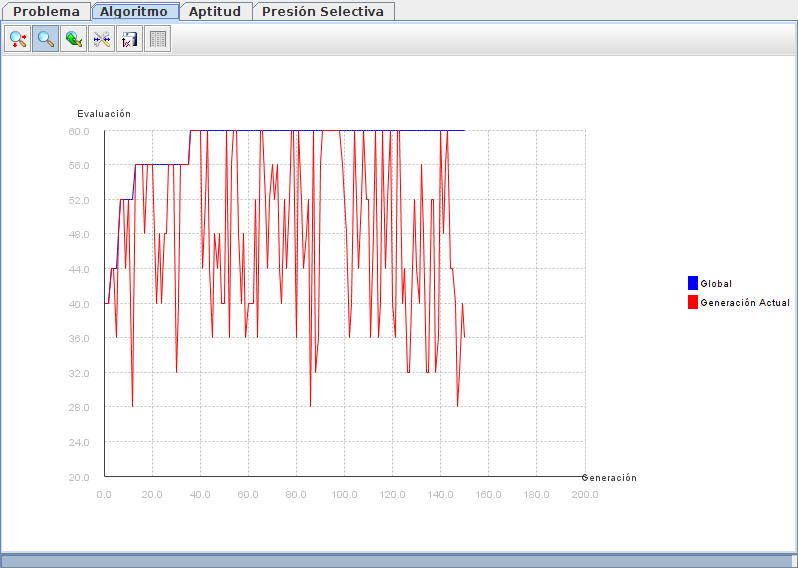
\includegraphics[scale=0.4]{graficas/pmg60}
\caption{Gráfica mejor resultado.}
\end{figure}

En la probabilidad de mutación sucede lo contrario que la probabilidad de cruce. Aquí se comporta mejor contra más pequeña es la probabilidad y se puede apreciar que con 0.05 nos da buenos resultados, al ir aumentando se pierde un poco la mejora pero siguen siendo buenos valores.	

	

\subsection{Porcentaje de Elitismo}
%tabla
\begin{table}[H]
\begin{center}
\begin{tabular}{|ccccc|} \hline
Porcentaje   & 0.0 & 0.02 & 0.1 & 0.3 \\  \hline
Resultado  &  52 & 56 & 56 & 64\\ \hline
\end{tabular}
\end{center}
\end{table}

\begin{figure}[H]
\centering
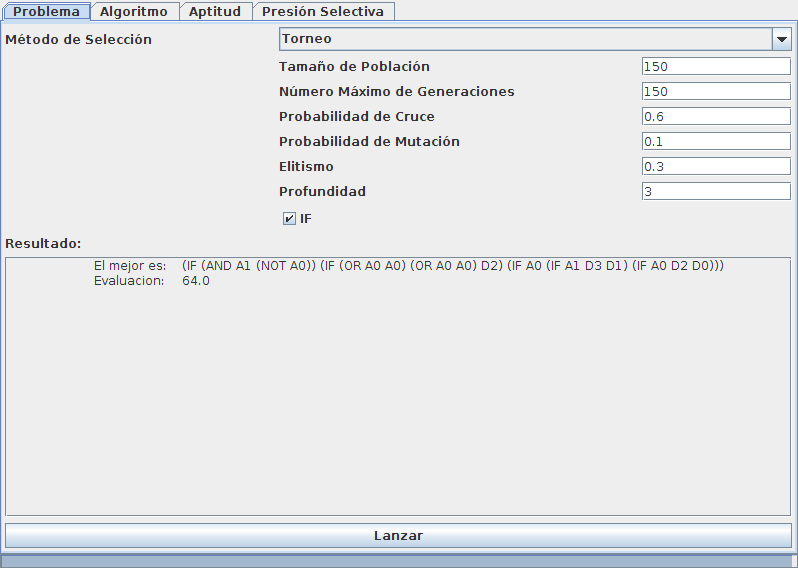
\includegraphics[scale=0.4]{graficas/e64}
\caption{Captura mejor resultado.}
\end{figure}

\begin{figure}[H]
\centering
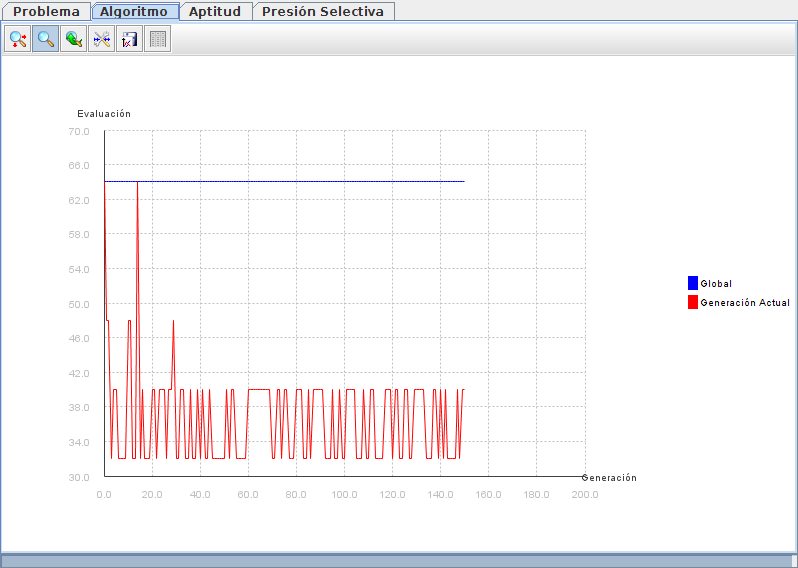
\includegraphics[scale=0.4]{graficas/eg64}
\caption{Gráfica mejor resultado.}
\end{figure}

EL elitismo se incluye para la mejora de nuestro algoritmo, al quedarse con los mejores de cada población cabe esperar una mejora de los resultados al aumentar dicho elitismo. En nuestras pruebas con un elitismo cercano a 0.3 nos da los mejores resultados.

\subsection{Profundidad}
%tabla
\begin{table}[H]
\begin{center}
\begin{tabular}{|ccccc|} \hline
Porcentaje   & 1 & 2 & 3 & 4 \\  \hline
Resultado  &  48 & 56 & 56 & 56\\ \hline
\end{tabular}
\end{center}
\end{table}

Referente a la profundidad con un 1 nivel no se pasa de 48 y al ir aumentando poco a poco se van dando mejores resultados pero haciendo media de ellos se nota un estancamiento a partir de 3 o 4 niveles, aumentando considerablemente el gasto de recursos de la maquina al tener que explorar mayor espacio de búsqueda. 

Por ultimo al probar el algoritmo sin la inclusión de la función IF el resultado baja notablemente hasta situarse cercano a 32. 

	


\section{Estudio de los diferentes parámetros del Algoritmo Genético con selección por Ranking}

	Estudio realizado con selección por ranking. Se han ido variando los diferentes parámetros, por defecto hemos tomados los siguientes valores:

%tabla
\begin{table}[H]
\begin{center}
\begin{tabular}{|cc|} \hline
Tamaño de la Población   & 150  \\  
Número Máximo de Generaciones  &  150 \\
Probabilidad de Cruce & 0.6 \\
Probabilidad de Mutación & 0.1 \\
Porcentaje de Elitismo & 0.1 \\
Profundidad & 3 \\ \hline
\end{tabular}
\end{center}
\end{table}


\subsection{Tamaño de la Población}

%tabla
\begin{table}[H]
\begin{center}
\begin{tabular}{|ccccc|} \hline
Tamaño	   & 50 & 100 & 150 & 200 \\  \hline
Resultado  &   &  &  &  \\ \hline
\end{tabular}
\end{center}
\end{table}

	

\subsection{Número Máximo de Generaciones}
%tabla
\begin{table}[H]
\begin{center}
\begin{tabular}{|ccccc|} \hline
Num Generaciones  & 100 & 200 & 300 & 400 \\  \hline
Resultado  &   &  &  &  \\ \hline
\end{tabular}
\end{center}
\end{table}	

	

\subsection{Probabilidad de Cruce}
%tabla
\begin{table}[H]
\begin{center}
\begin{tabular}{|ccccc|} \hline
Probabilidad   & 0.2 & 0.4 & 0.5 & 0.7 \\  \hline
Resultado  &  &  &  &  \\ \hline
\end{tabular}
\end{center}
\end{table}

	

\subsection{Probabilidad de Mutación}
%tabla
\begin{table}[H]
\begin{center}
\begin{tabular}{|ccccc|} \hline
Probabilidad   & 0.05 & 0.1 & 0.15 & 0.2 \\  \hline
Resultado  &   &  &  &  \\ \hline
\end{tabular}
\end{center}
\end{table}

	

\subsection{Porcentaje de Elitismo}
%tabla
\begin{table}[H]
\begin{center}
\begin{tabular}{|ccccc|} \hline
Porcentaje   & 0.0 & 0.02 & 0.1 & 0.3 \\  \hline
Resultado  &   &  &  &  \\ \hline
\end{tabular}
\end{center}
\end{table}


\section{Estudio de los diferentes parámetros del Algoritmo Genético con selección por Ruleta}

	Estudio realizado con selección por ruleta. Se han ido variando los diferentes parámetros, por defecto hemos tomados los siguientes valores:

%tabla
\begin{table}[H]
\begin{center}
\begin{tabular}{|cc|} \hline
Tamaño de la Población   & 100  \\  
Número Máximo de Generaciones  &  300 \\
Probabilidad de Cruce & 0.5 \\
Probabilidad de Mutación & 0.15 \\
Porcentaje de Elitismo & 0.02 \\ \hline
\end{tabular}
\end{center}
\end{table}


\subsection{Tamaño de la Población}

%tabla
\begin{table}[H]
\begin{center}
\begin{tabular}{|ccccc|} \hline
Tamaño	   & 50 & 100 & 150 & 200 \\  \hline
Resultado  &   &  &  &  \\ \hline
\end{tabular}
\end{center}
\end{table}

	

\subsection{Número Máximo de Generaciones}
%tabla
\begin{table}[H]
\begin{center}
\begin{tabular}{|ccccc|} \hline
Num Generaciones  & 100 & 200 & 300 & 400 \\  \hline
Resultado  &   &  &  & \\ \hline
\end{tabular}
\end{center}
\end{table}	

	

\subsection{Probabilidad de Cruce}
%tabla
\begin{table}[H]
\begin{center}
\begin{tabular}{|ccccc|} \hline
Probabilidad   & 0.2 & 0.4 & 0.5 & 0.7 \\  \hline
Resultado  &  &  &  &  \\ \hline
\end{tabular}
\end{center}
\end{table}

	

\subsection{Probabilidad de Mutación}
%tabla
\begin{table}[H]
\begin{center}
\begin{tabular}{|ccccc|} \hline
Probabilidad   & 0.05 & 0.1 & 0.15 & 0.2 \\  \hline
Resultado  &   &  &  &  \\ \hline
\end{tabular}
\end{center}
\end{table}

	

\subsection{Porcentaje de Elitismo}
%tabla
\begin{table}[H]
\begin{center}
\begin{tabular}{|ccccc|} \hline
Porcentaje   & 0.0 & 0.02 & 0.1 & 0.3 \\  \hline
Resultado  &  &  &  &  \\ \hline
\end{tabular}
\end{center}
\end{table}

	


\section{Conclusiones}

Primero se van a exponer las conclusiones relacionadas con los diferentes métodos de selección.

La selección por ruleta permite a los mejores individuos ser elegidos con una mayor probabilidad, pero también permite a los peores individuos ser elegidos, lo cual ayuda a mantener la diversidad de la población.
Un problema que hemos observado con los diferentes estudios realizados es que dicha selección hace perder diversidad y puede conducir a una convergencia prematura ya que la mayor parte de los individuos seleccionados serán una copia de los pocos predominantes.

En la selección por ranking los individuos se ordenan según su puntuación y luego son asignados con una segunda medida de puntuación, inversamente proporcional a su posición en el ranking. Los individuos son seleccionados proporcionalmente a esta probabilidad. Este método cómo se observa en los estudios realizados disminuye el riesgo de convergencia prematura que se produce cuando se utiliza selección de ruleta. Comentar que de los tres métodos implementados para la selección es el mas eficiente en cuanto a tiempo.

Por ultimo la selección por torneo se efectúa mediante una comparación entre un pequeño subconjunto de individuos elegidos al azar desde la población.
Los beneficios de este tipo de selección son la velocidad de aplicación ya que no es necesario evaluar ni comparar la totalidad de la población y la capacidad de prevenir la convergencia prematura. La principal desventaja es la necesidad de establecer el parámetro correspondiente al tamaño del subconjunto , en nuestro caso son 3 individuos y da buenos resultados.

Sobre las mejoras introducidas en la práctica hay que destacar el elitismo, método que copia los mejores individuos a la
próxima generación. El elitismo puede aumentar rápidamente hacia buenos individuos, ya que evita perder la mejor solución encontrada. Sin embargo,
es posible que este método haga converger rápidamente a un óptimo local.

Referente a la implementación de la práctica cabe destacar que hemos omitido la lectura por archivo de los 64 casos posibles del multiplexor utilizando una clase MUX que emula dicho comportamiento y contiene un método test para obtener nuestra aptitud de una manera más eficiente.

Cabe destacar un versión que probamos para buscar mas eficiencia a la hora de cruzar, consistía en ir creando un camino aleatorio en vez de hacer random y buscar ese nodo en el árbol, pero esta versión de búsqueda del punto del cruce no ofrecía variedad ya que se quedaba en los primeros niveles del árbol la mayoría de las veces por lo que decidimos desecharla.

\end{document}
